\documentclass[12pt,journal,compsoc]{IEEEtran}
\usepackage[utf8x]{inputenc}
\usepackage[portuguese]{babel}
\usepackage{listings}
\usepackage{graphicx}


\usepackage{color}

\definecolor{mygreen}{rgb}{0,0.6,0}
\definecolor{mygray}{rgb}{0.5,0.5,0.5}
\definecolor{mymauve}{rgb}{0.58,0,0.82}

\lstset{ %
	basicstyle=\ttfamily\footnotesize,
	backgroundcolor=\color{white},
	breakatwhitespace=false,
	breaklines=true,
	commentstyle=\color{mygreen},
	deletekeywords={...},
	escapeinside={\%*}{*)},
	extendedchars=true,
	% frame=single,
	keepspaces=true,
	keywordstyle=\color{blue},
	language=bash,
	morekeywords={cp},
	numbers=left,
	numbersep=2pt,
	numberstyle=\tiny\color{mygray},
	rulecolor=\color{black},
	showspaces=false,
	showstringspaces=false,
	showtabs=false,
	stepnumber=2,
	stringstyle=\color{mymauve},
	tabsize=2,
	title=\lstname
}

\hyphenation{op-tical net-works semi-conduc-tor}

\begin{document}
\title{Automação residencial:\\Comandando lâmpadas pelo \emph{Telegram}}

\author{\IEEEauthorblockN{Parley Martins - 11/0038096}
\IEEEauthorblockN{Tatielen Pereira - 12/0136074}
% \IEEEauthorblockA{Faculdade UnB Gama\\
% Universidade de Brasília\\
% Brasília, Brasil\\
% parleypachecomartins@gmail.com}
}

\IEEEcompsoctitleabstractindextext{%
\begin{abstract}
%\boldmath
Este trabalho propõe a utilização de automação residencial para possibilitar ao usuário acender e apagar lâmpadas remotamente, utilizando integração com aplicativo no celular.
\end{abstract}

\begin{IEEEkeywords}
Automação Residencial, Telegram, bot, \emph{smart house}
\end{IEEEkeywords}}

\maketitle

\section{Introdução}
% justificativa, objetivos, requisitos, benefícios, revisão bibliográfica).
Automação residencial é resultado da combinação de espaços residenciais, como sala, banheiro, quarto com tecnologias, para maior conforto, segurança, ou menos contato humano \cite{moraes2001using}. Estas tecnologias e ideias eram, até recentemente, consideradas sonhos de um futuro distante \cite{GHAFFARIANHOSEINI2013593}, sem uso prático, exceto no entretenimento.

No entanto com um mundo conectado pela internet, que mudou o jeito que as pessoas se comunicam e se relacionam, é normal que este conceito esteja cada vez mais próximo da realidade das pessoas. Para ter mais conforto, já é possível controlar pelo celular o volume das televisões (e outros aparelhos de som), o canal em que se está, a intensidade com que aparelhos devem funcionar, entre outras comodidades. Para ter mais segurança, é possível controlar luzes, sistema de alarmes, de detecção de movimentos, etc. Existem diversas empresas que fornecem esse tipo de serviço, mas eles ainda podem ter um custo muito elevado.

\section{Solução}

Para facilitar e desmistificar o acesso à automação residencial, a proposta deste projeto é implementar um sistema que possa controlar remotamente as lâmpadas de uma casa. O usuário, após instalação do sistema físico, poderá utilizar seu \emph{smartphone} para ligar e desligar as lâmpadas.

A interação com o usuário se dará através de um bot no aplicativo \emph{Telegram}. Deve-se iniciar uma 'conversa' com o bot, e mandar o comando desejado (ligar ou desligar, por exemplo). Este irá mandar para o módulo wifi do sistema, que fará a comunicação com o MSP, desligando ou ligando a lâmpada selecionada.

Para fins deste trabalho, uma lâmpada e uma fonte de energia externas, controladas pela protoboard, serão utilizadas para facilitar a instalação e testes.

O \textit{hardware} será composto, inicialmente, pelos seguintes items:

\begin{itemize}
\item protoboard, para execução do sistema;
\item microcontrolador MSP430, irá executar o controle da energia na lâmpada;
\item módulo esp8266, proverá o acesso à rede wifi;
\item lâmpada, para testes;
\item fonte de energia, tanto para o microcontrolador quanto para a lâmpada.
\end{itemize}

O \textit{software} embarcado no microcontrolador será escrito nas linguagens C e Assembly, enquanto o código do \textit{bot} será desenvolvido utilizando Python 3. Os serviços serão conectados através do IFTTT, que conecta servidores de terceiros a outros serviços \cite{ovadia2014automate}.

\subsection{Requisitos}

O \textit{software} do microcontrolador deve corretamente identicar os comandos e apagar ou acender a lâmpada, conforme instrução recebida.

O \emph{bot}, \textit{software} que responde a comandos pré definidos automaticamente, deve ser integrado ao aplicativo \textit{Telegram} e deve mandar instruções de ligar e de desligar a lâmpada.

O sistema completo, tanto hardware quanto \textit{software}, deve ter acesso à internet para o funcionamento correto.

\subsection{Benefícios}

Este projeto tem como principal beneficiário o cidadão comum que quer ter um pouco do conforto que a automação residencial traz a sua casa. Além disso, ajudará na economia de energia, já que a pessoa pode mandar um comando de apagar determinada luz, mesmo a distância.

\section{Desenvolvimento}

Esta seção apresenta um detalhamento do sistema proposto no projeto. Para isto, será apresentado a descrição do hardware e software.

\subsection{Hardware}

O Hardware utilizado pelo grupo consiste nos items descritos na Tabela \ref{tab:componentes}

\begin{table}[h!]
\centering
\caption{Tabela de componentes do projeto}
\label{tab:componentes}
\begin{tabular}{|l|c|}
\hline
Componentes & Quantidade \\ \hline
MSP430G2553 & 1 \\ \hline
Módulo Wireless ESP8266 & 1 \\ \hline
Protoboard  & 1 \\ \hline
Relé & 1 \\ \hline
Diodo & 1 \\ \hline
Lâmpada Led 12w  & 1 \\ \hline
Jumpers & Indefinido  \\ \hline
\end{tabular}
\end{table}

\begin{figure}[h!]
\centering
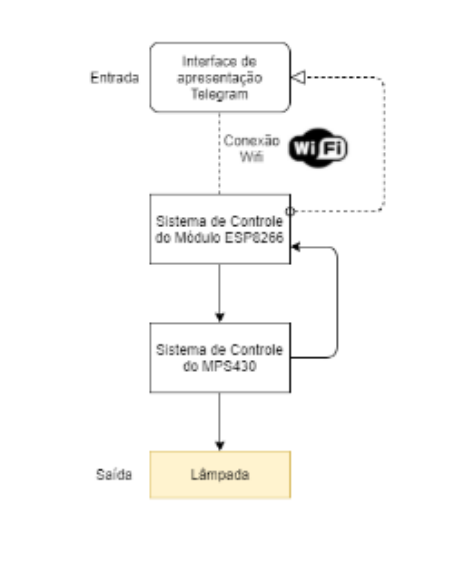
\includegraphics[width=200px,height=\textheight,keepaspectratio]{diagrama_blocos}
\caption{Diagrama de blocos do projeto}
\label{fig:diagrama_blocos}
\end{figure}

O diagrama de blocos tem como objetivo apresentar o princípio de funcionamento do sistema. Os blocos apresentados de acordo com a Figura \ref{fig:diagrama_blocos} são:


\begin{itemize}
\item \underline{Interface de apresentação} será o meio de comunicação entre o usuário e o sistema. Com o auxílio do aplicativo Telegram será possível escolher se o usuário acenderá, apagará ou verificar o estado em que a lâmpada se encontra.
\item \underline{Sistema de controle do módulo ESP8266} receberá a decisão enviada via aplicativo por conexão wifi para maior mobilidade do usuário. Como o usuário possui a possibilidade de verificar o estado da lâmpada o sistema de controle do módulo Wifi também envia um sinal de retorno para o app Telegram.
\item \underline{Sistema de controle do MSP430} será ligado junto ao módulo Wifi, onde será recebida e executada a decisão do usuário. Como o usuário possui a possibilidade de verificar o estado da lâmpada sistema de controle do MSP430 também envia um sinal de retorno para o módulo Wifi.
\item \underline{Lâmpada} será acesa dependendo da decisão do usuário.
\end{itemize}

Para conectar o módulo Wifi ESP8266 ao MSP430 foram conectados os seguintes pinos, de acordo com a Tabela \ref{tab:conexoes}. A lâmpada até o momento só foi testada com o LED 1 do próprio MSP.

\begin{table}[h!]
\centering
\caption{Tabela de conexoes MSP-ESP}
\label{tab:conexoes}
\begin{tabular}{|l|c|}
\hline
Módulo Wifi ESP8266 & MSP430 \\ \hline
TX & P1.4 \\ \hline
CH\_PD & VCC \\ \hline
RST &  \\ \hline
VCC & VCC \\ \hline
GND & GND \\ \hline
GPIO2 & \\ \hline
GPIO0 & \\ \hline
RX & P1.3 \\ \hline
\end{tabular}
\end{table}

O ESP foi configurado para se conectar à internet, mas não foi possível fazê-lo mandar dados para o MSP.

\subsection{Software}

O MSP foi configurado para receber um caractere na conexão UART que troca ou lê o estado da lâmpada. Os caracteres aceitos são \texttt{n}, para ligar; \texttt{f}, para desligar; e \texttt{s} para ler e retornar o estado atual da lâmpada. Qualquer outro input resultará em nenhum retorno ou ação do MSP. O código \ref{lst:lamp.c} inicializa o modo de comunicação UART com \textit{baud rate} 9600 e \textit{clock} em 1MHz. Caso algum dado seja recebido, uma interrupção do RX do UART será acionada. Esta interrupção lerá o valor recebido e tomará uma ação de acordo com o explicado acima. Para substituir a lâmpada, por enquanto, o LED conectado ao pino P1.6 do MSP está sendo utilizado.

\lstinputlisting[language=c, caption={\texttt{lamp.c}}, label=lst:lamp.c]{lamp.c}

O \textit{bot} do Telegram foi feito para responder à comandos pré-definidos. Após o uso de um deles, o \textit{bot} responde o usuário com uma mensagem de texto ou emoji, para demonstrar que o MSP recebeu e executou o comando, como demonstrado na Figura \ref{fig:telegram}.

\begin{itemize}
\item \texttt{/on}, vai ligar a lâmpada, retornando um emoji de lâmpada acesa.
\item \texttt{/off} desliga a lâmpada e retorna uma lua nova (pra demonstrar que a lâmpada foi apagada).
\item \texttt{/state} retorna o estado do lâmpada, com a mensagem "Light is {on/off}".
\end{itemize}

\begin{figure}[h!]
\centering
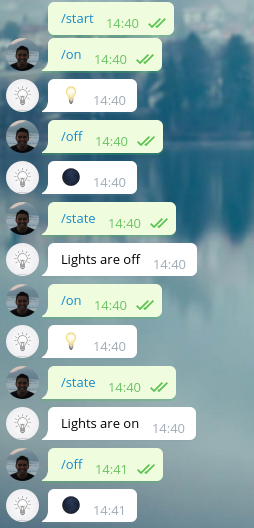
\includegraphics[width=200px,height=\textheight,keepaspectratio]{telegram_commands}
\caption{Comandos do Telegram}
\label{fig:telegram}
\end{figure}


\section{Resultados}

Para realizar a comunicação entre a internet e o MSP foi escolhido o modulo ESP 8266, no entanto, até este ponto do trabalho, a conexão entre eles não está totalmente pronta, pois comandos realizados em relação ao módulo wifi não estão gerando respostas satisfatórias. O ESP parece se conecta a internet, mas não devolve informações simples como o IP.


\section{Conclusão}



\bibliographystyle{IEEEtran}
\bibliography{IEEEabrv,bibliografia}

\end{document}
